% \usepackage{xcolor}
% \usepackage{afterpage}
% \usepackage{pifont,mdframed}
% \usepackage[bottom]{footmisc}

\makeatletter
\gdef\this@inputfilename{input.txt}
\gdef\this@outputfilename{output.txt}
\makeatother

\newcommand{\inputfile}{\texttt{input.txt}}
\newcommand{\outputfile}{\texttt{output.txt}}

\newenvironment{warning}
  {\par\begin{mdframed}[linewidth=2pt,linecolor=gray]%
    \begin{list}{}{\leftmargin=1cm
                   \labelwidth=\leftmargin}\item[\Large\ding{43}]}
  {\end{list}\end{mdframed}\par}
  
\noindent\begin{tabular}{ll}
\begin{minipage}[b]{0.8\textwidth}
Giorgio, per festeggiare il suo ennesimo compleanno, si è iscritto a un corso per sommelier, dove impara a distinguere ed apprezzare le diverse tipologie di vini. Si è accorto però che, nonostante prenda solo un assaggio di ogni tipo di vino, per lui vale la regola fondamentale delle bevande alcoliche: quando le bevi, mai scendere di gradazione. Infatti, se per esempio Giorgio assaggia un vino da 9 gradi e poi uno da 7, il giorno dopo si sveglierà con un grosso mal di testa indipendentemente dalle quantità.
Per fortuna, in ogni serata del corso è disponibile l’elenco dei vini che verranno portati uno dopo l’altro, e di ogni vino viene riportata la gradazione alcolica. Non è ammesso mettere da parte un vino per berlo in seguito: ogni volta che gli viene passato un vino Giorgio può decidere se assaggiarlo o meno, versandone un poco nel suo Tastevin. Inoltre, dal momento che dopo aver assaggiato un vino Giorgio deve pulire accuratamente il suo Tastevin con un panno, questa operazione in pratica gli impedisce di assaggiare due vini consecutivi (nell’immagine qui a fianco potete vedere il Tastevin). Giorgio desidera assaggiare il maggior numero di vini possibile. 
\end{minipage}
&
\begin{minipage}[t]{3cm}
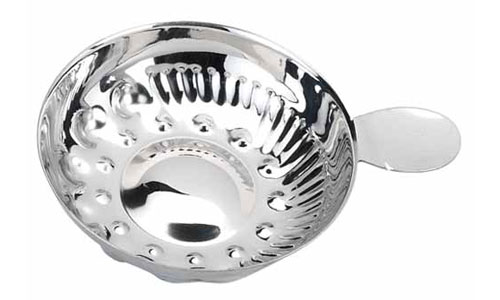
\includegraphics[width=3cm]{tastevin.jpg}\\
\vspace{0.1cm}
\end{minipage} 
\end{tabular}

\begin{tabular}{|c|c|c|c|c|c|c|c|c|}
\hline 1 & 2 & 3 & 4 & 5 & 6 & 7 & 8 & 9 \\
\hline Cilento & Barolo & Lambrusco & Picolit & Verdicchio & Cannonau & Chianti & Pigato & Donzelle \\ 
\hline 11 & 13 & 10 & 16 & 12 & 12 & 13 & 11 & 13\\
\hline
\end{tabular}

Ad esempio, se in una serata serviranno i vini mostrati nella tabella qui sopra, nell’ordine in cui compaiono nella tabella,  il numero massimo di vini che Giorgio può riuscire ad assaggiare, rispettando la regola, è quattro: può iniziare, indifferentemente, con il Cilento o con il Lambrusco, e poi assaggiare Verdicchio, Chianti e Donzelle. In questa maniera, la sequenza delle gradazioni alcoliche non scende mai: 11 (oppure 10), 12, 13, 13. Ovviamente, come si vede nell’esempio, è possibile bere due o più vini con la stessa gradazione alcolica.

\InputFile
Il file \inputfile{} è composto da 2 righe. La prima riga contiene $N$, un intero positivo: il numero di vini che saranno serviti nella serata. La seconda riga contiene $N$ interi positivi: le gradazioni alcoliche dei vini che saranno serviti, nell’ordine in cui saranno serviti.

\OutputFile
Il file \outputfile{} è composto da una sola riga contenente un solo intero positivo: il numero massimo di vini che Giorgio può assaggiare nella serata, rispettando la regola di non diminuire la gradazione alcolica nella sequenza e, contemporaneamente, il vincolo di dover pulire il Tastevin, che gli impedisce di assaggiare due vini consecutivi.

\pagebreak
\Implementation
Dovrai sottoporre esattamente un file con estensione \texttt{.c}, \texttt{.cpp} o \texttt{.pas}.

\begin{warning}
Tra gli allegati a questo task troverai un template (\texttt{sommelier.c}, \texttt{sommelier.cpp}, \texttt{sommelier.pas}) con un esempio di implementazione da completare.
\end{warning}

Se sceglierai di utilizzare il template, dovrai implementare la seguente funzione:
\begin{center}\begin{tabularx}{\textwidth}{|c|X|}
\hline
C/C++  & \verb|int degusta(int N, int *V);|\\
\hline
Pascal & \verb|function degusta(N: longint; var V: array of longint): longint;|\\
\hline
\end{tabularx}\end{center}
In cui:
\begin{itemize}[nolistsep]
  \item L'intero $N$ rappresenta il numero di vini.
  \item L'array \texttt{V}, indicizzato da $0$ a $N-1$, contiene le gradazioni alcoliche dei vini, nell'ordine in cui sono serviti.
  \item La funzione dovrà restituire la risposta al problema, che verrà stampata sul file di output.
\end{itemize}

% Assunzioni
\Constraints
\begin{itemize}[nolistsep, itemsep=2mm]
\item $1 \le N \le 10\,000$.
\item I vini hanno una gradazione alcolica compresa tra 1 e 99.
\end{itemize}

\Scoring
Il tuo programma verrà testato su diversi test case raggruppati in subtask.
Per ottenere il punteggio relativo ad un subtask, è necessario risolvere
correttamente tutti i test relativi ad esso.

\begin{itemize}[nolistsep,itemsep=2mm]
  \item \textbf{\makebox[2cm][l]{Subtask 1} [10 punti]}: Casi d'esempio.
  \item \textbf{\makebox[2cm][l]{Subtask 2} [20 punti]}: $N \leq 10$.
  \item \textbf{\makebox[2cm][l]{Subtask 3} [40 punti]}: $N \leq 100$.
  \item \textbf{\makebox[2cm][l]{Subtask 4} [30 punti]}: Nessuna limitazione specifica.
\end{itemize}

% Esempi
\Examples
\begin{example}
\exmp{
9

11 13 10 16 12 12 13 11 13
}{%
4
}%
\end{example}
\begin{example}
\exmp{
12

11 13 11 10 11 12 16 12 12 11 10 14 
}{%
5
}%
\end{example}

\end{document}
